\documentclass{standalone}

\usepackage{tikz}
\usepackage{amsmath}
\usepackage{xstring} 
\usetikzlibrary{decorations.pathreplacing}
\usetikzlibrary{fadings}
\usetikzlibrary{fit,positioning}
\usetikzlibrary{shapes.geometric}

\newcommand\drawNodes[2]{
  % #1 (str): namespace
  % #2 (list[list[str]]): list of labels to print in the node of each neuron
  \foreach \neurons [count=\lyrIdx] in #2 {
    \StrCount{\neurons}{,}[\arrlength] % uses the xstring package
    \foreach \n [count=\nIdx] in \neurons
      \node[neuron] (#1-\lyrIdx-\nIdx) at (2*\lyrIdx, \arrlength/2-1*\nIdx) {\n};
  }
}

\newcommand\denselyConnectNodes[2]{
  % #1 (str): namespace
  % #2 (list[int]): number of nodes in each layer
  \foreach \n [count=\lyrIdx, remember=\lyrIdx as \previdx, remember=\n as \prevn] in #2 {
    \foreach \y in {1,...,\n} {
      \ifnum \lyrIdx > 1
        \foreach \x in {1,...,\prevn}
          \draw[->] (#1-\previdx-\x) -- (#1-\lyrIdx-\y);
      \fi
    }
  }
}

\begin{document}
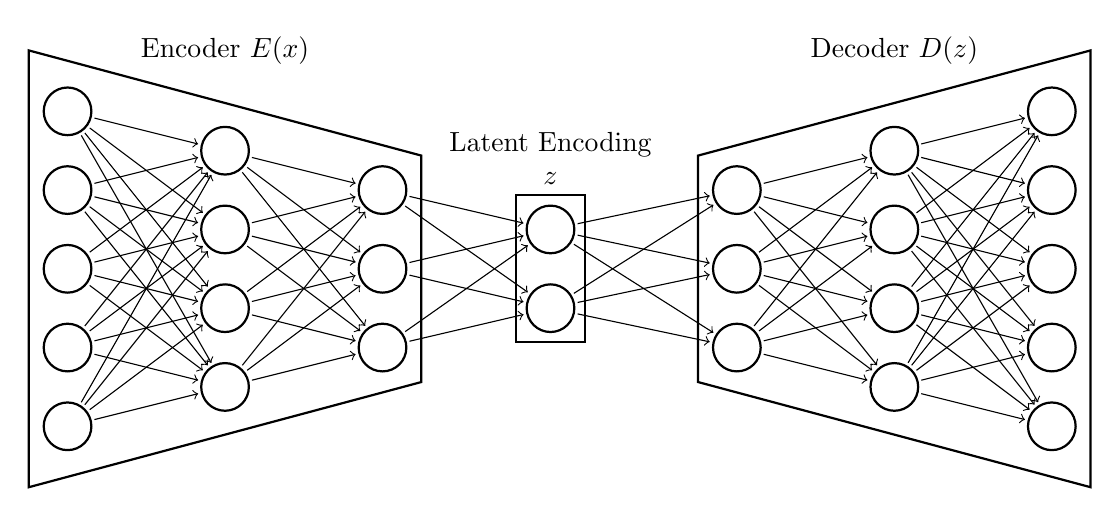
\begin{tikzpicture}[
    shorten >=1pt, shorten <=1pt,
    neuron/.style={circle, draw, minimum size=4ex, thick},
    legend/.style={font=\large\bfseries},
  ]

  % encoder
  \drawNodes{encoder}{{{,,,,}, {,,,}, {,,}}}
  \denselyConnectNodes{encoder}{{5, 4, 3}}

  % decoder
  \begin{scope}[xshift=8.5cm]
    \drawNodes{decoder}{{{,,}, {,,,}, {,,,,}}}
    \denselyConnectNodes{decoder}{{3, 4, 5}}
  \end{scope}

  % mu, sigma, sample nodes
  \foreach \idx  in {1,2} {
      \coordinate[neuron, right=1.5 of encoder-3-2, yshift=\idx cm-1.5cm, fill opacity=0.2] (mu\idx);
    %   \coordinate[neuron, right=2 of encoder-3-2, yshift=-\idx cm, fill=blue, fill opacity=0.1] (sigma\idx);
    }

  % mu, sigma, sample boxes
  \node [label={[align=center]Latent Encoding\\$z$}, fit=(mu1) (mu2), draw, opacity=1, thick] (mu) {};
  \node [trapezium, label=left:{Encoder $E({x})$}, trapezium angle=75, fit=(encoder-3-1) (encoder-3-3) (encoder-1-1) (encoder-1-5), draw, rotate=-90, opacity=0.45, thick, inner xsep=-25pt, inner ysep=5pt, outer sep=10pt, opacity=1, thick] (encode) {};
  \node [trapezium, label=right:Decoder $D({z})$, trapezium angle=75, fit=(decoder-1-1) (decoder-1-3) (decoder-3-1) (decoder-3-5), draw, rotate=90, opacity=0.45, thick, inner xsep=-25pt, inner ysep=5pt, outer sep=10pt, opacity=1,thick] (decode) {};
%   \node [label=$\sigma$, fit=(sigma1) (sigma3), draw, fill=blue, opacity=0.3] (sigma) {};
%   \node [label=sample, fit=(sample1) (sample2, draw, fill=green, opacity=0.3] (sample) {};

%   % mu, sigma, sample connections
%   \draw[->] (mu.east) -- (sample.west);
  \foreach \a in {1,2,3}
	\foreach \b in {1,2} {
		\draw[->] (encoder-3-\a) -- (mu\b);
		\draw[->] (mu\b) -- (decoder-1-\a);
		% \draw[->] (encoder-3-\a) -- (sigma\b);
		% \draw[->] (sample\a) -- (decoder-1-\b);
    }

  % input + output labels
%   \foreach \idx in {1,...,5} {
%       \node[left=0 of encoder-1-\idx] {$x_\idx$};
%       \node[right=0 of decoder-3-\idx] {$\hat x_\idx$};
%     }

\end{tikzpicture}
\end{document}